\section{Research method} 

Gregor \cite{gregor2006nature}, gives “A Taxonomy of Theory Types in Information Systems Research”. 
To answer our research questions we will conduct what she calls “Type V: Theory for Design and Action”. 
The criteria for success of this type of research “include utility to a community of users, the novelty of the artefact, and the persuasiveness of claims that it is effective”.

To do this we will apply projectional editing techniques, through the MPS language workbench to the Drools language.
We have observed the difficulty with which developers are having to reason about and edit large collections of Drools files.
We hypothesize that developers can be presented with different views on their code that will allow them to better understand the code.
The novelty of our approach will be to create new view types specific to the needs of a Drools programmer.

We will be relying on MPS as well as other open source components to work together with acceptable performance such that the user experience is acceptable.
Figure \ref{fig:MPS_IDE} shows the JetBrains open source IDE for MPS. 
In this you create the Concepts, Generators, Type Systems, etc., that are necessary to define the language.
You also create editors, which gives your language out of the box IDE support.

\begin{figure}[H]
    \centering
    \fbox{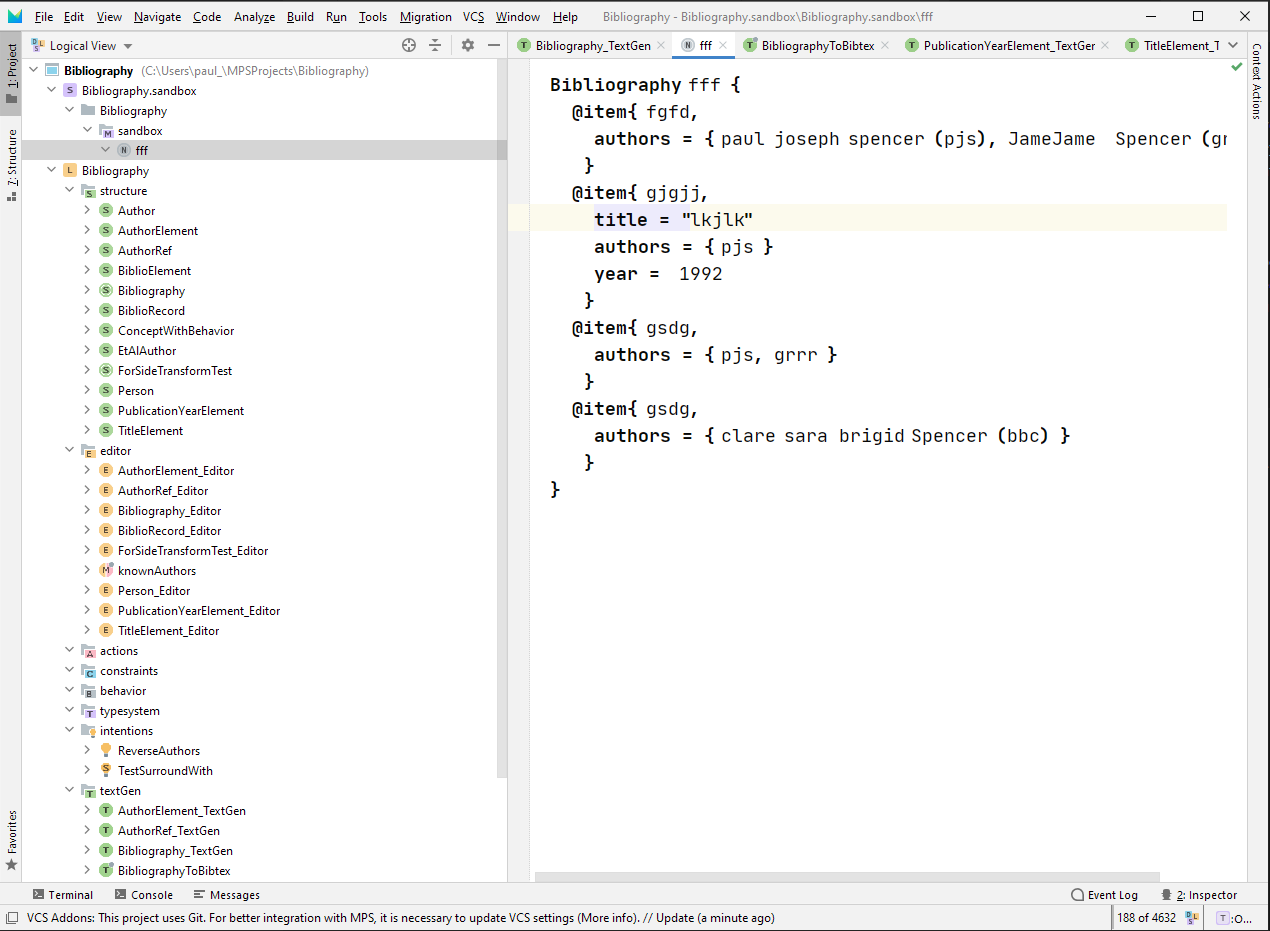
\includegraphics[width=0.95\textwidth]{images/MPS_IDE.png}}
    \caption{MPS IDE}
    \label{fig:MPS_IDE}
\end{figure}

The projection design, which will run in parallel to the Drools language modelling, will depend in part on the outcome of research carried out in the first period.

Whether our design is appropriate with regards to performance and functionality is a risk. 
Also the usefulness of the projections is a risk.
This is where I expect to gain the biggest benefit of literature review and academic supervision. 

The major tasks in this prototype development will be: 
\begin{itemize}
    \item Modelling the Drools language.
    \item Developing the alternative projections.
\end{itemize}

The prototype itself will be validated by working.
However, if time permits, the hypothesis of the usefulness of the projections will be validated through developer use surveys.

{\LARGE TO REMOVE}

Present how you are going to find the answers to your research question. This section should cover:
\begin{itemize}
    \item What will make the research difficult?
    \item What is the input you expect from the literature survey
    \item What sources will you use and how will you use / document them?
    \item What experiments / research will you do? What proof of concept will you make?
	\item What method will you use?
\end{itemize}